\documentclass[../main.tex]{subfiles}
\begin{document}
\subsection{The superconducting diode effect}
\subsubsection{A classical diode working scheme}
    A diode is a ubiquitous component of electric circuits. It has two poles and allows the current to flow in one direction only, cf. Fig\ref{fig:iv-diode-SDE} (left). 
    Let us consider one semiconductor that has been doped with an excess of electrons (n-doped) and another one with an excess of 
    holes (p-doped). Both material are neutral. One now brings them together at an interface. First due to diffusion, some electron from the n-doped material leak
    inside the p-doped one. The concentration of electron is in fact smaller there. The same happens for the holes, see Fig.\ref{fig:diode} (top left).

    An electron enters the p region and will after some time scatters from the conduction band to the valence band of the dopant, because it is energetically more favorable. 
    The electron and hole recombine.
    This leaves a region around the interface free of charge carriers:
    the depletion region, see Fig.\ref{fig:diode} (top right). The new-acquired valence electron does not contribute to transport but
    still carries a charge. We therefor have a negatively charged lattice on the p-side of the depletion band. Further, we have a
    positively charged lattice on the n-side of the depletion band (the conducting electrons left their donator atoms). 
    Due to the charge density gradient in the vicinity of the interface, there is an electric field forming that works against the diffusion.
    It prevents further charge carrier leakage between the two semiconductors. 

    We now connect the n side with the positive part of a potential source and the p side with the negative one (reversed bias).  The conduction electrons (and holes) are
    pulled away from the interface, ionizing more doping atoms by leaving. Therefore, the depletion region widens, and the junction works like an
    insulator. The drift caused by the field in the depletion region overcomes the diffusion, and it is very unlikely for an electron to make it to the p-doped material, compare Fig.\ref{fig:diode} (left).  The opposite applies for the holes.
    By reversing the polarity (forward bias), the electrons are attracted towards the junction and fill the space electron left free when diffusing to the interface
    in the zero bias case. The depletion region narrows, and the diffusion can now most likely bring the electrons across the interface. They then recombine 
    with holes in the p-doped material. This also happens for the holes, so that the two of them move in opposite direction with opposite charge, yielding
    a net current. The diode now let the current flow, cf. Fig.\ref{fig:diode} (right).
    
    \begin{figure}[H]
        \centering
        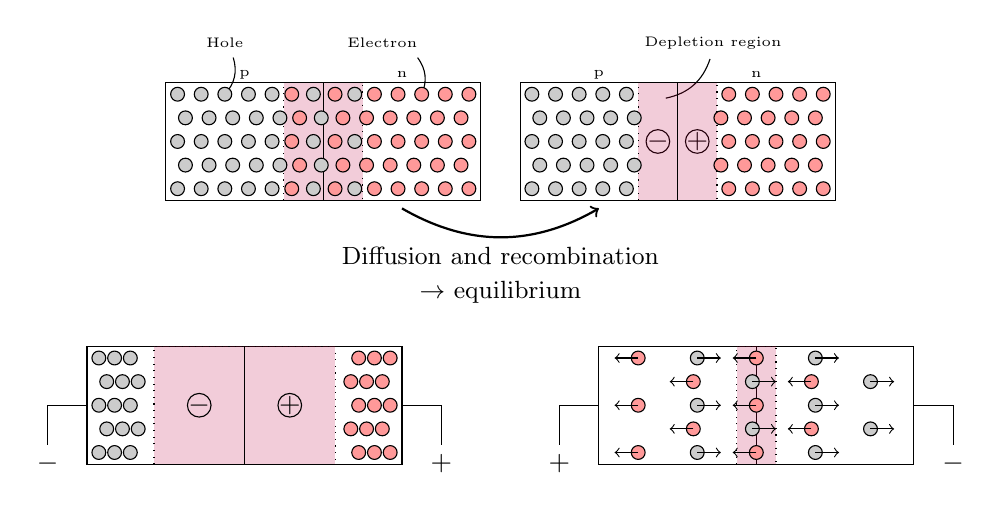
\begin{tikzpicture}[darkstyle/.style={circle,draw,fill=gray!40,minimum size=5pt, inner sep=0pt},
            lightstyle/.style={circle,draw,fill=red!40,minimum size=5pt, inner sep=0pt}]
            \draw[fill=purple, fill opacity=0.2, dotted] (-1.5-2.25,0) rectangle ++(1,1.5);
            \draw[draw=black,-] (-1-2.25,0)-- ++(0,1.5);
            \draw[draw=black] (-5.25,0) rectangle ++(4,1.5);
            \node (elec) at (-2.5,2) {\tiny Electron};
            \node (hole) at (-4.5,2) {\tiny Hole};
            \node (depl) at (1.7,2) {\tiny Depletion region};
            \path[-] (1.1,1.3) edge[bend right] (depl);
            \node at (-4.25,1.6) {\tiny p};
            \node at (-2.25,1.6) {\tiny n};
            \node at (0.25,1.6) {\tiny p};
            \node at (2.25,1.6) {\tiny n};
            \draw (1.5,0.75) circle (0.15) node {$+$};
            \draw (1,0.75) circle (0.15) node {$-$};
            \path[-] ({ -2.85 -2.25+0.3*2},0.15+1.2) edge[bend right] (hole);
            \path[-] ({ +0.85-2.25-0.3*2},0.15+1.2) edge[bend right] (elec);
            % \draw[thick,<-] (0.75,-0.15) -- (1.75,-0.15)
            %     node[midway, below] {$E$};
            \foreach \x in {0,...,4}
                \foreach \y in {0,...,4} {
                    \node[darkstyle] at
                    ({0.3*\x + 0.1*mod(\y,2) -2.85 -2.25}, {0.3*\y + 0.15}) {};
                    \node[lightstyle] at
                    ({-0.3*\x - 0.1*mod(\y,2) +0.85-2.25}, {0.3*\y + 0.15}) {};
                    }

            \foreach \x in {0,...,2}
                \foreach \y in {0,...,4}{
                    \pgfmathtruncatemacro{\result}{mod(\x,2)}

                    \ifnum\result=1
                        \node[darkstyle] at ({0.275*\x-1.4+0.1*mod(\y,2)-2.25},0.3*\y+ 0.15) {};
                    \else
                        \node[lightstyle] at ({0.275*\x-1.4+0.1*mod(\y,2)-2.25},0.3*\y+ 0.15) {};
                    \fi}
                \foreach \y in {0,...,2} \node[darkstyle] at ( -0.6-2.25, {0.6*\y + 0.15}) {};

            \draw[fill=purple, fill opacity=0.2, dotted] (-1.5+2.25,0) rectangle ++(1,1.5);
            \draw[draw=black,-] (-1+2.25,0)-- ++(0,1.5);
            \path[thick,->] (-2.25,-0.1) edge[bend right] node [below, align=center] {\small
                Diffusion and recombination\\
                \small$\rightarrow$ equilibrium
                } (0.25,-0.1);

            \draw[draw=black] (-3+2.25,0) rectangle ++(4,1.5);
            \foreach \x in {0,...,4}
                \foreach \y in {0,...,4} {
                    \node[darkstyle] at
                    ({0.3*\x + 0.1*mod(\y,2) -2.85 +2.25}, {0.3*\y + 0.15}) {};
                    \node[lightstyle] at
                    ({-0.3*\x - 0.1*mod(\y,2) +0.85+2.25}, {0.3*\y + 0.15}) {};
                    }

        \begin{scope}[shift={(0,-1.5)}]
            \draw[draw=black] (-6.25,-1.85) rectangle ++(4,1.5);
            \draw[fill=purple, fill opacity=0.2, dotted] (-5.4,-1.85) rectangle ++(2.3,1.5);
            \draw (-3.675,-1.1) circle (0.15) node {$+$};
            \draw (-4.825,-1.1) circle (0.15) node {$-$};

            \draw[draw=black,-] (-4.25,-1.85)-- ++(0,1.5);
            \draw[draw=black,-] (-6.25,-1.1)-- ++(-0.5,0);
            \draw[draw=black,-] (-6.75,-1.1)-- ++(0,-0.5) node[below] {\(-\)};

            \draw[draw=black,-] (-2.25,-1.1)-- ++(0.5,0);
            \draw[draw=black,-] (-1.75,-1.1)-- ++(0,-0.5) node[below] {\(+\)};

            \foreach \x in {0,...,2}
                \foreach \y in {0,...,4} {
                    \node[darkstyle] at
                    ({0.2*\x + 0.1*mod(\y,2) -6.1}, {0.3*\y + 0.15-1.85}) {};
                    \node[lightstyle] at
                    ({-0.2*\x - 0.1*mod(\y,2) -2.4}, {0.3*\y + 0.15-1.85}) {};
                    }


            \draw[draw=black] (0.25,-1.85) rectangle ++(4,1.5);
            \draw[draw=black,-] (2.25,-1.85)-- ++(0,1.5);
            \draw[fill=purple, fill opacity=0.2, dotted] (2,-1.85) rectangle ++(0.5,1.5);
            \draw[draw=black,-] (-4.25,-1.85)-- ++(0,1.5);
            \draw[draw=black,-] (0.25,-1.1)-- ++(-0.5,0);
            \draw[draw=black,-] (-0.25,-1.1)-- ++(0,-0.5) node[below] {\(+\)};

            \draw[draw=black,-] (4.25,-1.1)-- ++(0.5,0);
            \draw[draw=black,-] (4.75,-1.1)-- ++(0,-0.5) node[below] {\(-\)};

          \foreach \x in {0,...,3}
                \foreach \y in {0,...,4}{
                    \pgfmathtruncatemacro{\result}{mod(\x,2)}

                    \ifnum\result=1
                        \node[darkstyle] at ({0.75*\x+0.5+0.7*mod(\y,2)+0.25},0.3*\y+ 0.15-1.85) {};
                        \draw[->,thin] ({0.75*\x+0.5+0.7*mod(\y,2)+0.25},0.3*\y+ 0.15-1.85) --++(0.3,0);
                    \else
                        \node[lightstyle] at ({0.75*\x+0.5+0.7*mod(\y,2)+0.25}, 0.3*\y+ 0.15-1.85) {};
                        \draw[->,thin] ({0.75*\x+0.5+0.7*mod(\y,2)+0.25}, 0.3*\y+ 0.15-1.85) -- ++(-0.3,0);
                    \fi}

            % \draw[thick,->] (1.25,-2) -- (3.25,-2)
            %     node[midway, below] {$E$};

            % \draw[thick,<-] (-5.25,-2) -- (-3.25,-2)
            %     node[midway, below] {$E$};
        % \path[use as bounding box] (-7,-4.5) rectangle (0,0);
            \end{scope}
        \end{tikzpicture}
        \caption{(Top) the electrons and holes at equilibrium after bringing the p and n dotted material at an interface. The depletion region appears.
            (Left) the reversed direction where the current is blocked. (Right) the forward direction lets the current flow. See text.
        }
        \label{fig:diode}
    \end{figure}
\subsection{Superconducting diode}
In a superconductor we have no electric resistivity. However, when we leave the superconducting phase by applying too much temperature or magnetic field,
the superconductivity breaks and the standard IV-characteristic of the metal is back. A superconducting diode is superconducting for current $I_1$ and
is in the normal state for $I_2 = -I_1$. Therefor, the current $I_1$ flows without resistivity and $I_2$ gets partially blocked.  They are the same current with opposite 
polarity.  So the superconducting diode need an asymmetry in its IV-characteristic, cf. Fig\ref{fig:iv-diode-SDE} (right).

\begin{figure}
    \centering
    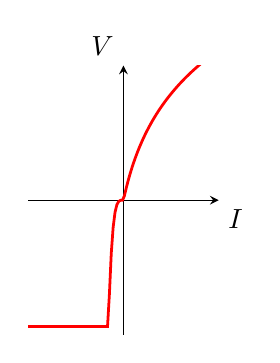
\begin{tikzpicture}
\begin{axis}[
    width=4cm,
    height=5cm,
    axis lines=center,
    xlabel={$I$},
    ylabel={$V$},
    xlabel style={below right},
    ylabel style={above left},
    xtick=\empty,
    ytick=\empty,
    ymin = -1.7,
    ymax = 1.7,
    xmin = -1.7,
    xmax = 1.7,
]
    \addplot[
        color=red,
        line width=1pt,
        % domain=-1.5:1.5,
        samples=300,
    ]
    {x>0 ? ln(x+0.3)-ln(0.3) : (x>-0.27 ? -300*x^4 : -1.595)};
\end{axis}
    \end{tikzpicture}
    \hspace{48pt}
        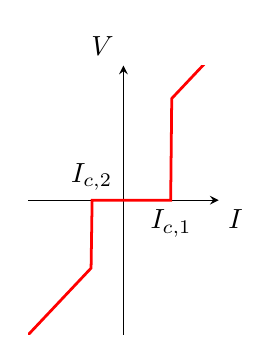
\begin{tikzpicture}
\begin{axis}[
    width=4cm,
    height=5cm,
    axis lines=center,
    xlabel={$I$},
    ylabel={$V$},
    xlabel style={below right},
    ylabel style={above left},
    xtick=\empty,
    ytick=\empty,
    ymin = -4,
    ymax = 4,
    xmin = -3,
    xmax = 3,
]
    \addplot[
        color=red,
        line width=1pt,
        % domain=-3:3,
        samples=300,
    ]
    {(x < -1) ? (x-1) : ((x > 1.5) ? (x+1.5) : 0)};
 \node[anchor=north, color=black] at (axis cs:1.5,0) {\(I_{c,1}\)};
  \node[anchor=south, color=black] at (axis cs:-1,0) {\(I_{c,2}\)};
\end{axis}

    \end{tikzpicture}
    \caption{(Left) the IV-curve of a np-junction. For the forward bias $V>0$ the voltage $V$ is an exponential of the current $I$. At reversed bias $V<0$ the $I$ remains negligible and for 
    high enough voltage, the breakdown happens, where the depletion region is overcome, and the current can flow despite gap.
    (Right) the IV-characteristic of a superconducting diode effect. In between the critical current $I_{c,1}$ and $I_{c,2}$ the diode is superconducting and has vanishing resistance. 
    In the other cases it follows the IV curve of a normal metal. When there is an asymmetry $|I_{c,1}|\neq|I_{c,2}|$ then the diode is superconducting or normal conducting for two current
    sign of the same amplitude. Inspired by Ref.\cite{Nadeem2023-jj}.
     }
    \label{fig:iv-diode-SDE}
\end{figure}



\end{document}